
%% This LaTeX-file was created by <gquinn> Mon Dec  8 06:23:18 2003
%% LyX 0.12 (C) 1995-1998 by Matthias Ettrich and the LyX Team

%% Do not edit this file unless you know what you are doing.
\documentclass[reqno,12pt]{amsart}
\usepackage[T1]{fontenc}
\usepackage{graphicx}
\usepackage{hyperref}

\begin{document}
\vspace{3 cm}
\begin{center}
\textbf{\Large{RICAS IRT Model}}
\end{center}
\vspace{1 cm}

\section*{Structure of the IRT Model}
Item Response Theory (IRT) is a collection of psychometric models that are widely used to standardize and model the results of tests that measure student achievement and/or ability.  This type of model has been in use in education for at least fifty years.
\par\vspace{0.3 cm}
Usually an IRT model assumes that, for a given student, the probability that they will correctly answer a specific item is a function of an ability parameter ($\theta$) associated with the student together with a set of parameters known as the \textit{IRT parameters} associated with that test item.  
\par\vspace{0.3 cm}
The formulas for computing the probability of a correct response given $\theta$ and the IRT parameters are documented in the 2018 MCAS and MCAS-Alt Technical Report, Section 3.6.1. \cite{ngtr} 
\par\vspace{0.3 cm}

For each item on the test, the IRT parameters are estimated during the test calibration process.  For the 2018 RICAS, the IRT parameter estimates are posted on the Massachusetts Department of Elementary and Secondary Education's website. \cite{irtp}.
\par\vspace{0.3 cm}
The $\theta$ values are assumed to have a standard normal distribution in the population (i.e., a bell curve distribution with mean zero and standard deviation one).
\subsection*{Dichotomous Items} 
Dichotomous items receive a score of either one or zero depending on the answer the student gives.
\par\vspace{0.3 cm}
A three-parameter logistic (3PL) model is used for dichotomous items.  For each item and student, the probability that the student receives a score of 1 is determined by the values of the three IRT parameters:
\begin{itemize}
\item $a$ discrimination 
\item $b$ difficulty 
\item $c$ pseudo guessing
\end{itemize}
in combination with the student ability parameter $\theta$ and a normalizing constant $D$ whose value is 1.701.
\par\vspace{0.3 cm}
The formula for computing the probability of receiving a score of $1$ on item $i$ given $a_i,b_i,c_i$ and $D$ for student $j$ with ability parameter $\theta_j$ is:
\vspace{0.5 cm}
\[
P_i(1|\theta_j,a_i,b_i,c_i) = c_i + (1-c_i)\left(\frac{\exp\left[Da_i(\theta_j-b_i)\right]}{1+\exp\left[Da_i(\theta_j-b_i)\right]}\right)
\vspace{0.5 cm}
\] 
Example: Item IA00323 from the 2018 ELA Grade 3 test (paper version) has the following estimated parameter values: (\cite{irtp} p.22)
\begin{itemize}
\item $a$ (discrimination) = 1.06404
\item $b$ (difficulty)     = -0.76098
\item $c$ (pseudo guessing) = 0.13650
\end{itemize}
\par\vspace{0.3 cm}
For a student at the median ability in the population ($\theta=0$), the probability of a correct answer on this item is predicted to be:
\[
0.13650 + (1-0.13650)\left(\frac{\exp\left[1.701\cdot 1.06404(0+0.76098)\right]}{1+\exp\left[1.701\cdot 1.06404(0+0.76098)\right]}\right) = .826
\vspace{0.5 cm}
\]
For a student at the $25^{th}$ percentile of the ability distribution ($\theta=-0.67$), the formulas assigns the probability $0.604$ to a correct answer.
\par\vspace{0.3 cm}
The difficulty parameter $b$ is low for this item, indicating that it is relatively easy.
\par\vspace{0.3 cm}
As the ability parameter $\theta$ varies from $-3$ to $3$, the probability a correct answer varies from approximately zero to approximately one, along an S=shaped curve similar to the one in the figure:
\vspace{0.5 cm}
\begin{center}
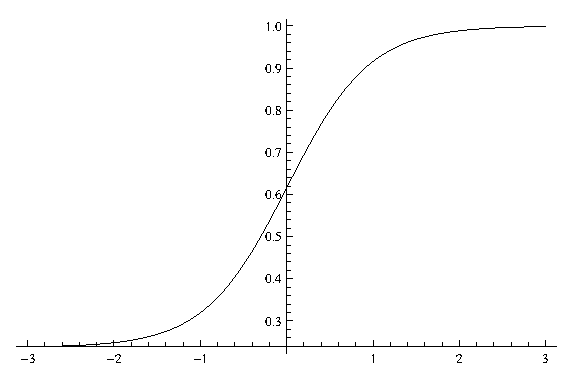
\includegraphics[width=9cm,height=5cm]{RICAS_IRT_model_fig1.eps}
\end{center}
\par\vspace{0.3 cm}
If you draw a horizontal line segment with length $1$ on the graph from $y=0$ to $y=1$ at any value of $\theta$ on the horizontal axis, the portion of that line that is above the curve is the probability of an incorrect answer, and the portion below the graph is the probability of a correct answer. 
\par\vspace{0.3 cm}
Most of the items on the RICAS are dichotomous, but there are a few that can receive scores other than zero or one.  These are called \textit{polytomous} items.  These have more than three IRT parameters, and a more complicated probability formula, but the formula still produces a predicted probability for each possible score. 
\section*{How we might use this}
It is my understanding that RIDE does not currently have a psychometrician on staff, so I think we have an opportunity for East Greenwich to take the lead on using this information. 
\par\vspace{0.3 cm}
Using the individual item level scores for every student, it should be possible to produce an extimate of that student's $\theta$ value (with a confidence interval), which we could then use to compute the probability of a correct answer on each item. 
\par\vspace{0.3 cm}
If a student missed a question that they had a low probability of answering correctly, one could argue that they performed about as expected.
\par\vspace{0.3 cm}
On the othere hand, if they miss a question that the model says they should have a high probability of answering correctly, then that could be interpreted to be an indication that they were not adequately prepared on the part of the curriculum the item tested.  
\par\vspace{0.3 cm}
Educators could use that information to tailor individual instruction targeting the student's weaknesses. 

\begin{thebibliography}{99}

\bibitem{ngtr} \href{http://www.mcasservicecenter.com/documents/MA/Technical%20Report/2018/NextGen/2018%20MCAS%20NextGen%20Technical%20Report.pdf}{MCAS 2018 NextGen Technical Report}: Section 3.6.1, p.54
\vspace{0.5 cm}  
\bibitem{irtp} Table M-3:Next Generation MCAS and MCAS Alt: IRT Parameters for Dichotomous Items - ELA Grade 3 Paper. MCAS 2018 NextGen Technical Report:   \href{http://www.mcasservicecenter.com/documents/MA/Technical%20Report/2018/NextGen/Appendix M-Plots and IRT Parameters.pdf}{Appendix M - Plots and IRT Parameters}

\end{thebibliography}
\end{document}

